\documentclass[11pt]{article}
\newcommand{\tb}{\textbf}
\usepackage{fullpage}
\usepackage{hyperref}
\usepackage{amssymb}
\usepackage{spalign}
\usepackage{amsmath}
\usepackage{framed}
\newcommand{\R}{\mathbb{R}}
\usepackage[parfill]{parskip}

\usepackage{graphicx}
\graphicspath{./figures/}
\setcounter{tocdepth}{2}

\hbadness=99999

\hypersetup{
    colorlinks,
    citecolor=black,
    filecolor=black,
    linkcolor=black,
    urlcolor=black
}
\urlstyle{urlcolor=blue}

\newcommand{\contradiction}{%
  \ensuremath{{\Rightarrow\mspace{-2mu}\Leftarrow}}%
}

\newcommand{\then}{\rightarrow}

\newtheorem{theorem}{Theorem}[section]
\newtheorem{definition}[theorem]{Definition}
\newtheorem{axiom}[theorem]{Axiom}
\newtheorem{example}[theorem]{Example}

\renewcommand{\contentsname}{Table of Contents}
\title{Logic and Set Theory}
\author{Sidharth Baskaran}

\begin{document}
\maketitle

% \tableofcontents
% \newpage
% -------------------------------------

\section{Common Sense Reasoning (Bonevac)}

\begin{itemize}  
    \item Thoughts are organized by general principle, 
    e.g. acids being corrosive, what goes up must come down.
    \item Are not \textbf{universal or necessary} as they have exceptions.
    Thus, inference from principle to conclusions are not deductively valid.
    \item To formalize principles, need to be able to draw conclusions from them but also withdraw these
    with further information. Classical logic does not allow for widthdrawable conclusions, for a valid argument does not need to
    revalidated-\textbf{guarantees} truth of its conclusion.
    \item Thus, need a system of logic to reach \textit{defeasible} conclusions-reasonable but defeatable with further info
    \item Classical logic is monotonic-if set $S$ implies conclusion $\mathcal{B}$, then any set with all of $S$ also implies $\mathcal{B}$, so adding premises cannot make valid argument invalid
    \item New system of logic is non-monotonic, adding premises can sometimes make invalid argument
\end{itemize}

\subsection{Good arguments going bad}

Can add a premise to a deductively invalid argument to make it valid. A conditional always works.

\begin{example}
    Invalid: Mt. Everest is there. So Mt. Everest should be climbed.\newline
    With premise: Mt. Everest is there. \textbf{If it is there, it should be climbed.} So Mt. Everest should be climbed.
\end{example}

\begin{itemize} 
    \item A deductively valid argument cannot be invalidated with additional premises
    \item An argument is valid if the truth of premises guarantees truth of conclusion, so if the premises are true the conclusion \textbf{must} be true, \textit{but also if} falsity of premises implies falsity of conclusions
    \item In real-world arguments, premise cannot guarantee truth of conclusion. Additional information may cause withdrawal of inference.
    \begin{itemize}
        \item Validity doesn't require the truth of the premises, instead it merely necessitates that conclusion follows from the formers without violating the correctness of the logical form
    \end{itemize}
    \item An argument can be deductively invalid but inductively valid, or \textit{defeasibly valid/allowed}, so premises \textit{defeasibly imply} conclusion.
    \begin{itemize}
        \item Argument is defeasibly valid iff premises are true \textbf{and} reasonable to expect conclusion to be true.
    \end{itemize}
    \item Precisely term this as a \textbf{counterexample}, circumstance in which premises are true but conclusion false
\end{itemize}

\section{Abstraction and truth functional logic}

\begin{itemize} 
    \item Use \textit{atomic sentences} (e.g. $A$ or $B$) to express information as a statement, whereas the statement is its \textit{extension}.
    Always are capital letters and are simplest way to express information.
    \item Use parentheses in truth-functional expressions to clearly convey information
\end{itemize}

\begin{definition}[Case]
    A case is a particular assignment of truth values to atomic sentences. $n$ atomic sentences correspond to $2^n$ cases.
\end{definition}

\begin{definition}[Principle of Excluded Middle]
    The principle of the excluded middle says that given a sentence, either it or the negation is true in any case.
\end{definition}

\begin{definition}[Principle of Non-Contradiction]
    A sentence and its negation can't be true in the same case.
\end{definition}

\subsection{Logical Operators}

\begin{center}
\begin{tabular}[]{|c|c|c|}
    \tb{Operator} & \tb{Name} & \tb{Vernacular equivalent}\\
    \hline
    $\lnot$ & negation & not\\
    $\land$ & conjunction & and, but, although\\
    $\lor$ & disjunction & or\\
    $\then$ & conditional & if-then, only if\\
    $\leftrightarrow$ & biconditional & iff, necessary + sufficient, exactly when
\end{tabular}
\end{center}

The English word \textit{unless} can be translated as a conditional, but there is a trick in interpretation. 
Take example of {\color{red} The patient will die ($A$) unless we operate ($B$)}. 
The correct translation is $\lnot B\then A$, \textbf{not} $B\then \lnot A$. This is due to the definition of the conditional; 
we cannot say that $B\leftrightarrow \lnot A$ or the inverse isn't true. Surgery does not \ti{guarantee} the patient living, but we know that if we don't operate, the patient will surely die.

Further note that using the equivalence conditional disjunction equivalence theorem, $(\lnot B\then A)\leftrightarrow (B\lor A)$.
So we can also interpret unless as a simple disjunction.

\begin{figure}[H]
    \centering
    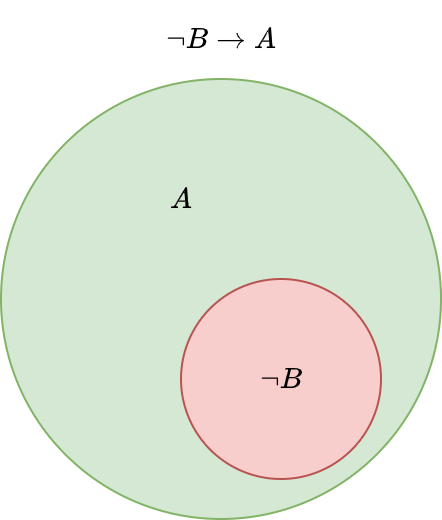
\includegraphics[scale=0.4]{figures/venn-conditional.png}
    \caption{Visualization of conditional}
\end{figure}

\section{Arguments}

\begin{itemize} 
    \item Consists of a non-negative number of premises along with one conclusion
    \item Premise is a sentence, just like conclusion
    \item Standard form lists premises, followed by horizontal line (therefore) and the conclusion
    \item Logic assesses \textit{validity} of arguments and we can see if the argument is \textit{sound}
\end{itemize}

\begin{definition}[Validity]
    An argument is valid iff every case in which all its premises are true forces the conclusion to be true.
\end{definition}

\begin{definition} [Soundness]
    An argument is sound iff it is valid and premises are actually true (i.e. in real life).
\end{definition}

\begin{definition}[Counterexample]
    A case in which an argument's premises are all true but the conclusion is false.
\end{definition}

A valid argument therefore has a relaxed definition; it is only invalid if there exists a counterexample to it.

\subsection{Arguments and theorems}

\begin{definition}[Tautology]
    A sentence if a tautology iff it is true in all cases.
\end{definition}

\begin{definition}[Contingent]
    A contingent sentence is true in some cases and false in others.
\end{definition}

\begin{definition}[Contradiction]
    Sentence of the form $A\land \lnot A$, so it is always false. The sentences $A$ and $\lnot A$ are \tb{contradictory}.
\end{definition}

\begin{definition}[Consistent]
    A set of sentences is consistent iff there is a case where all of them are true. So for $n$ sentences $\{A_1,A_2,\ldots A_n\}$, $A_1\land A_2\land A_3\ldots \land A_n$ is true for \tb{at least one case}.
\end{definition}

\begin{definition}[Argument-theorem exchange]
    The argument\\
    
    \begin{center}
        \begin{tabular}{c}
            $P_1$\\$P_2$\\$P_3$\\\vdots\\$P_n$\\\hline\\C
        \end{tabular}
    \end{center}

    is valid iff $(P_1\land P_2\land P_3\ldots \land P_n)\then C$ is a tautology.
\end{definition}

\section{Common Fallacies (Bennett)}

\begin{itemize} 
    \item \textbf{Error of Conversion}. Can't affirm the antecedent given the premise that affirms the consequent. In other words, given $\{p\then q,q\}$ as premises, cannot conclude that $p$ is true.
    \item \textbf{Error of Inversion}. Denying the antecedent and incorrectly denying the consequent. In the premises $p$ is not true then $q$ is true, $p$ is not true, incorrect to conclude that $q$ is not true.
\end{itemize}

\section{Informal proof}

Formal proofs are computationally verified (e.g. truth table) and informal proofs fall in one of below categories.
The below methodology is to prove validity of an argument.

\subsection{Conditional proof}

Assume premises are true. Use light of reasoning to show that conclusion is also true in such a case. Conclude that argument is valid. Is sufficient to prove validity because by assuming the premises, we show that the conclusion must follow, or be implied.

\subsection{Proof by contradiction}

Assume there exists a counterexample (true premises and a false conclusion). Show this assumption leads to a contradiction. Then conclude that the argument is valid.
Notably, this method is effective at proving \textbf{disproving} arguments, because when assuming the existence of a counterexample, you either reach a contradiction or affirm its existence–sufficient for a disproof.

\section{Logical Equivalences and Inference}

\begin{tabular}{l|l|l}
    \tb{Name} & \tb {Tautology} & \tb{Code} \\
    \hline \hline Conditional Disjunction & $(A \rightarrow B) \leftrightarrow(\neg A \vee B)$ & CDis \\
    Contraposition & $(A \rightarrow B) \leftrightarrow(\neg B \rightarrow \neg A)$ & ContraPos \\
    Definition of Equivalence & $(A \leftrightarrow B) \leftrightarrow((A \rightarrow B) \wedge(B \rightarrow A))$ & Equiv \\
    DeMorgan's Law (1) & $\neg(A \wedge B) \leftrightarrow(\neg A \vee \neg B)$ & DeM \\
    DeMorgan's Law (2) & $\neg(A \vee B) \leftrightarrow(\neg A \wedge \neg B)$ & DeM \\
    Distribution of And over Or & $(A \wedge(B \vee C)) \leftrightarrow((A \wedge B) \vee(A \wedge C))$ & Distr \\
    Distribution of Or over And & $(A \vee(B \wedge C)) \leftrightarrow((A \vee B) \wedge(A \vee C))$ & Distr \\
    Double Negation & $\neg \neg A \leftrightarrow A$ & DN \\
    Repetition & $(A \vee A) \leftrightarrow A$ & Rep\\
\end{tabular}

Also, commute sentences over $\wedge, \mathrm{V}$, and $\leftrightarrow$.
Final operator applied in evaluation is the \textbf{main operator}.

\begin{tabular}{l|l|l}
    \tb{Name} & \tb {Inference} & \tb{Code} \\
    \hline \hline Addition & From $A$, infer $A \vee B(B$ may be any sentence) & Add \\
    Conjunction & From $\{A, B\}$, infer $A \wedge B$ & Conj \\
    Constructive Dilemma & From $\{A \vee B, A \rightarrow C, B \rightarrow D\}$, infer $C \vee D$ & $\mathrm{CD}$ \\
    Contradictory Premises & From $\{A, \neg A\}$, infer $B(B$ may be any sentence) & ContraPrm \\
    Disjunctive Syllogism & From $\{A \vee B, \neg A\}$, infer $B$ & DS \\
    Hypothetical Syllogism & From $\{A \rightarrow B, B \rightarrow C\}$, infer $A \rightarrow C$ & HS \\
    Modus Ponens & From $\{A \rightarrow B, A\}$, infer $B$ & MP \\
    Simplification & From $A \wedge B$, infer $A$ & Simp \\
    Tautology & Infer $A \vee \neg A(A$ may be any sentence) & Taut\\
\end{tabular}

\section{Natural deduction}

Begin by listing \textbf{premises}, then apply set of logical equivalences
or rules of inference to arrive at the \textbf{conclusion}. See 1.6 of Textbook
for equivalences and inference rules.

% -------------------------------------
\end{document}